\subsection{Speisung}
\label{subsec:Speisung}

\subsubsection{3.3V-Spannung}
Um die Speisung des Analog- bzw. des Digital-Teils zu verifizieren wurde die Spannung nach den jeweiligen LDOs mit einem Agilent 34410A Multimeter gemessen. Die USB-Versorgungs-Spannung schwankt je nach Quelle zwischen 4.9 und 5.2V, jedoch sollte sie nach den LDOs konstant 3.3V betragen. Gemessen wurden folgende Spannungen:

\begin{equation}
V_{dd_{analog}}=3.2924\si{V}
\end{equation}

\begin{equation}
V_{dd_{digital}}=3.2957\si{V}
\end{equation}

Weiter wurden die Spitzen der Spannungsversorgung mit einem Tektronix TDS 2014C Oszilloskop gemessen. Als Vergleich einmal vom Stromnetz und einmal von einer handelsüblichen Powerbank gespiesen.

\begin{figure} [H]
\begin{minipage}[c]{0.45\textwidth}
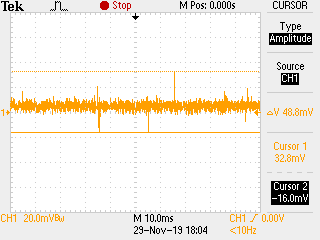
\includegraphics[width=\textwidth]{graphics/Speisung_Netz_Analog.png}
\end{minipage}
\begin{minipage}[c]{0.45\textwidth}
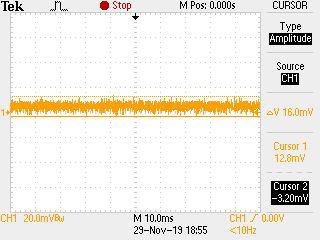
\includegraphics[width=\textwidth]{graphics/Speisung_PB_Analog.png}
\end{minipage}
\caption{Vergleich der analogen Speisung am Netz (links) und mit einer Powerbank (rechts)}
\label{fig:analogspeisung}
\end{figure} 

\begin{figure} [H]
\begin{minipage}[c]{0.45\textwidth}
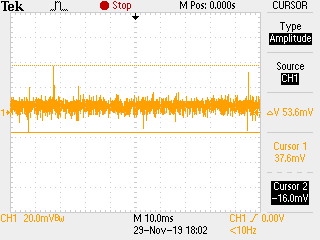
\includegraphics[width=\textwidth]{graphics/Speisung_Netz_Digital.png}
\end{minipage}
\begin{minipage}[c]{0.45\textwidth}
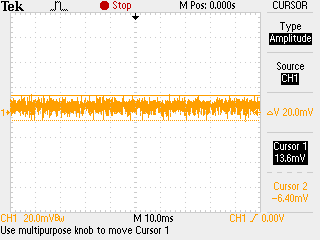
\includegraphics[width=\textwidth]{graphics/Speisung_PB_Digital.png}
\end{minipage}
\caption{Vergleich der digitalen Speisung am Netz (links) und mit einer Powerbank (rechts)}
\label{fig:digitalspeisung}
\end{figure} 

Wie in Abbildungen \ref{fig:analogspeisung} und \ref{fig:digitalspeisung} ersichtlich macht die unterschiedliche Speisung vom Netz sowie der Powerbank einen Unterschied in den Spannungsspitzen. Die Spitzen erreichen 50mV Peak-Peak, was jedoch von den Stützkondensatoren am Microcontroller und am Codec geglättet wird. Das Grundrauschen der Spannung von 20mV ist vertretbar. Die Speisung funktioniert wie erwartet.

\subsubsection{Stromverbrauch}
\label{sec:Valid_Stromverbrauch}

Die Stromaufnahme der gesamten Schaltung über den Akkumulator wurde mit Hilfe einer Source Measuring Unit (SMU) ermittelt.
Für die Messung lief das DSP Board mit der Demo Software. Beide OLED Displays zeigten Text, die FPU ist eingeschaltet und berechnet ein FIR Filter. Es waren keine Audioquellen oder -senken verbunden.

\begin{table}[H]
	\begin{tabular}{|l|l|l|c|c|}
		\hline
		Messgerät      & Kanal & Prüffmittelnummer & Spannungsbereich & Strombegrenzung \\ \hline
		Agilent N6705B & CH1   & MSZ-M-0064        & 3.7V - 4.2V      & 0.2A            \\ \hline
	\end{tabular}
	\caption{Parameter der SMU}
	\label{tab:SMU_Params}
\end{table}

Der über den gesamten Spannungsbereich von $3.7\si{V}$ bis  $4.2\si{V}$ gemessene Stromverbrauch beläuft sich auf:

\begin{equation}
I_{bat}=64\si{mA}
\end{equation}

Die Stromaufnahme bleibt über den Spannungsbereich konstant, weil die Schaltung die Leistung an der Betriebsspannung von $3.3\si{V}$ konstant bleibt. 
Der Stromfluss durch die LDO's bleibt gleich. Einzig die Verlustleistung an den LDO's steigt mit einer höherer Batteriespannung.



